% answers.tex —— 2020 年·新高考Ⅰ卷（山东） · 参考答案与详细解析片段
% 由 tools/generate_projects.py 依来源总账自 2020/2020_数学真题_新高考1_试题.md + 2020/2020_数学真题_新高考1_解析正文.md + 2020/2020_数学真题_新高考1_答案要点.md 生成，勿手改（改源 MD 后重跑）


\begin{answer}
\gksolhead{1}{}

\textbf{题目}：

设集合 $A=\{x\mid 1\leqslant x\leqslant 3\}$，$B=\{x\mid 2<x<4\}$，则 $A\cup B=$\mbox{（　　）}

（A）$\{x\mid 2<x\leqslant 3\}$；（B）$\{x\mid 2\leqslant x\leqslant 3\}$；（C）$\{x\mid 1\leqslant x<4\}$；（D）$\{x\mid 1<x<4\}$。

\Needspace{4\baselineskip}
\textbf{解析}

\Needspace{5\baselineskip}
$A=\{x\mid1\leqslant x\leqslant3\}=[1,3]$，$B=\{x\mid2<x<4\}=(2,4)$。两者在数轴上首尾相接：$A$ 的左端点 $1$ 保留，$B$ 的右端点 $4$ 不取，中间 $[1,3]$ 与 $(2,4)$ 有重叠部分 $(2,3]$，合起来恰是一整段
\nopagebreak[4]
\[A\cup B=[1,4)=\{x\mid1\leqslant x<4\}.\]

也可以正反两面说清：一方面 $A\subseteq[1,4)$、$B\subseteq[1,4)$，故 $A\cup B\subseteq[1,4)$；另一方面若 $1\leqslant x<4$，则当 $x\leqslant3$ 时 $x\in A$，当 $x>3$ 时 $x>2$ 且 $x<4$，$x\in B$，故 $[1,4)\subseteq A\cup B$。

逐项核对：（A）丢了 $[1,2]$ 与 $(3,4)$；（B）只剩 $[2,3]$；（D）丢了 $x=1$；只有（C）与 $[1,4)$ 完全一致。

选 C。

\gkanswer{答案：C。$A=[1,3]$，$B=(2,4)$，并集为 $[1,4)$，即 $\{x\mid1\leqslant x<4\}$。}

\end{answer}
\begin{answer}
\gksolhead{2}{}

\textbf{题目}：

$\dfrac{2-\mathrm i}{1+2\mathrm i}=$\mbox{（　　）}

（A）$1$；（B）$-1$；（C）$\mathrm i$；（D）$-\mathrm i$。

\Needspace{4\baselineskip}
\textbf{解析}

\Needspace{5\baselineskip}
分子分母同乘分母的共轭复数 $1-2\mathrm i$。先算分母：
\nopagebreak[4]
\[(1+2\mathrm i)(1-2\mathrm i)=1^2-(2\mathrm i)^2=1+4=5 .\]
\Needspace{5\baselineskip}
再算分子：
\nopagebreak[4]
\[(2-\mathrm i)(1-2\mathrm i)=2-4\mathrm i-\mathrm i+2\mathrm i^2=2-5\mathrm i-2=-5\mathrm i .\]
\Needspace{5\baselineskip}
故
\nopagebreak[4]
\[\frac{2-\mathrm i}{1+2\mathrm i}=\frac{-5\mathrm i}{5}=-\mathrm i .\]

选 D。

\gkanswer{答案：D。$\dfrac{2-\mathrm i}{1+2\mathrm i}=\dfrac{(2-\mathrm i)(1-2\mathrm i)}5=\dfrac{-5\mathrm i}5=-\mathrm i$。}

\end{answer}
\begin{answer}
\gksolhead{3}{}

\textbf{题目}：

$6$ 名同学到甲、乙、丙三个场馆做志愿者，每名同学只去 $1$ 个场馆，甲场馆安排 $1$ 名，乙场馆安排 $2$ 名，丙场馆安排 $3$ 名，则不同的安排方法共有\mbox{（　　）}

（A）$120$ 种；（B）$90$ 种；（C）$60$ 种；（D）$30$ 种。

\Needspace{4\baselineskip}
\textbf{解析}

\Needspace{5\baselineskip}
三个场馆的容量固定为 $1$、$2$、$3$，只要确定「哪 $1$ 人去甲、哪 $2$ 人去乙」，剩下 $3$ 人自然全去丙，故为分步组合计数：
\nopagebreak[4]
\[\mathrm C_6^1\cdot\mathrm C_5^2\cdot\mathrm C_3^3=6\times10\times1=60 .\]
也可按「先分组再分配」理解：人数型 $1+2+3$ 的分组数为 $\dfrac{6!}{1!\,2!\,3!}=60$，而三组人数互不相同，分到甲、乙、丙只有 $1$ 种对应方式，故仍是 $60$。

选 C。

\gkanswer{答案：C。先给甲馆选 $1$ 人、再给乙馆选 $2$ 人，余下 $3$ 人进丙馆：$\mathrm C_6^1\mathrm C_5^2\mathrm C_3^3=6\times10\times1=60$。}

\end{answer}
\begin{answer}
\gksolhead{4}{}

\textbf{题目}：

日晷是中国古代用来测定时间的仪器，利用与晷面垂直的晷针投射到晷面的影子来测定时间。把地球看成一个球（球心记为 $O$），地球上一点 $A$ 的纬度是指 $OA$ 与地球赤道所在平面所成角，点 $A$ 处的水平面是指过点 $A$ 且与 $OA$ 垂直的平面。在点 $A$ 处放置一个日晷，若晷面与赤道所在平面平行，点 $A$ 处的纬度为北纬 $40^\circ$，则晷针与点 $A$ 处的水平面所成角为\mbox{（　　）}

[第4题图：原页为日晷实景照片，按本库「实景照片不重绘、不入图」规则不入图，题干信息已完整照录]

（A）$20^\circ$；（B）$40^\circ$；（C）$50^\circ$；（D）$90^\circ$。

\Needspace{4\baselineskip}
\textbf{解析}

\Needspace{5\baselineskip}
记晷针所在直线为 $n$。由「晷针与晷面垂直」「晷面与赤道所在平面平行」得
\nopagebreak[4]
\[n\perp\text{\text{赤道所在平面}},\]
即晷针平行于地轴。

\Needspace{5\baselineskip}
设赤道所在平面的法线为地轴方向。点 $A$ 的纬度为 $40^\circ$，即 $OA$ 与赤道所在平面成 $40^\circ$ 角，于是 $OA$ 与地轴（赤道平面的法线）的夹角为
\nopagebreak[4]
\[90^\circ-40^\circ=50^\circ .\]
\Needspace{5\baselineskip}
又点 $A$ 处的水平面与 $OA$ 垂直，即水平面的法线沿 $OA$ 方向，故晷针与水平面所成角为
\nopagebreak[4]
\[90^\circ-50^\circ=40^\circ .\]

换个说法：晷针与水平面所成角恰等于「地轴与水平面所成角」，而后者正是当地纬度（北极星的地平高度等于纬度），故为 $40^\circ$。

选 B。

\gkanswer{答案：B。晷针 $\perp$ 晷面 $\parallel$ 赤道面，故晷针平行于地轴；地轴与水平面所成角等于当地纬度 $40^\circ$。}

\end{answer}
\begin{answer}
\gksolhead{5}{}

\textbf{题目}：

某中学的学生积极参加体育锻炼，其中有 $96\%$ 的学生喜欢足球或游泳，$60\%$ 的学生喜欢足球，$82\%$ 的学生喜欢游泳，则该中学既喜欢足球又喜欢游泳的学生数占该校学生总数的比例是\mbox{（　　）}

（A）$62\%$；（B）$56\%$；（C）$46\%$；（D）$42\%$。

\Needspace{4\baselineskip}
\textbf{解析}

\Needspace{5\baselineskip}
记 $F$ 为「喜欢足球」的学生集合，$S$ 为「喜欢游泳」的学生集合，用比例代替人数（全体学生记为 $1$）。已知
\nopagebreak[4]
\[|F\cup S|=96\%,\qquad |F|=60\%,\qquad |S|=82\% .\]
\Needspace{5\baselineskip}
由容斥原理
\nopagebreak[4]
\[|F\cap S|=|F|+|S|-|F\cup S|=60\%+82\%-96\%=46\% .\]

于是既喜欢足球又喜欢游泳的学生占 $46\%$。合理性检查：$46\%\leqslant\min\{60\%,82\%\}$，且 $60\%-46\%=14\%$、$82\%-46\%=36\%$、都不喜欢的为 $1-96\%=4\%$，于是「只喜欢足球」「只喜欢游泳」「都不喜欢」三项合计 $14\%+36\%+4\%=54\%=1-46\%$，自洽。

选 C。

\gkanswer{答案：C。由容斥原理，既喜欢足球又喜欢游泳的比例为 $60\%+82\%-96\%=46\%$。}

\end{answer}
\begin{answer}
\gksolhead{6}{}

\textbf{题目}：

基本再生数 $R_0$ 与世代间隔 $T$ 是新冠肺炎的流行病学基本参数。基本再生数指一个感染者传染的平均人数，世代间隔指相邻两代间传染所需的平均时间。在新冠肺炎疫情初始阶段，可以用指数模型：$I(t)=\mathrm e^{rt}$ 描述累计感染病例数 $I(t)$ 随时间 $t$（单位：天）的变化规律，指数增长率 $r$ 与 $R_0$，$T$ 近似满足 $R_0=1+rT$。有学者基于已有数据估计出 $R_0=3.28$，$T=6$。据此，在新冠肺炎疫情初始阶段，累计感染病例数增加 $1$ 倍需要的时间约为（$\ln2\approx0.69$）\mbox{（　　）}

（A）$1.2$ 天；（B）$1.8$ 天；（C）$2.5$ 天；（D）$3.5$ 天。

\Needspace{4\baselineskip}
\textbf{解析}

\Needspace{5\baselineskip}
先由 $R_0=1+rT$ 求指数增长率：
\nopagebreak[4]
\[r=\frac{R_0-1}{T}=\frac{3.28-1}{6}=\frac{2.28}6=0.38 .\]
\Needspace{5\baselineskip}
「累计感染病例数增加 $1$ 倍」即 $I(t)=2I(0)$，由 $I(t)=\mathrm e^{rt}$ 得
\nopagebreak[4]
\[\mathrm e^{rt}=2\ \Longrightarrow\ rt=\ln2\ \Longrightarrow\ t=\frac{\ln2}{r}=\frac{0.69}{0.38}\approx1.8158 .\]
与选项对照，最接近的是 $1.8$ 天（误差 $0.016$ 天；其余选项 $1.2$、$2.5$、$3.5$ 分别对应 $r\approx0.575$、$0.276$、$0.197$，与 $0.38$ 相差甚远）。

选 B。

\gkanswer{答案：B。$r=\dfrac{R_0-1}T=\dfrac{2.28}6=0.38$，加倍时间 $t=\dfrac{\ln2}r=\dfrac{0.69}{0.38}\approx1.8$（天）。}

\end{answer}
\begin{answer}
\gksolhead{7}{}

\textbf{题目}：

已知 $P$ 是边长为 $2$ 的正六边形 $ABCDEF$ 内的一点，则 $\overrightarrow{AP}\cdot\overrightarrow{AB}$ 的取值范围是\mbox{（　　）}

（A）$(-2,6)$；（B）$(-6,2)$；（C）$(-2,4)$；（D）$(-4,6)$。

\Needspace{4\baselineskip}
\textbf{解析}

\Needspace{5\baselineskip}
建立平面直角坐标系：取 $A$ 为原点，$\overrightarrow{AB}$ 方向为 $x$ 轴正方向。边长为 $2$ 的正六边形顶点依次为
\nopagebreak[4]
\[A(0,0),\ B(2,0),\ C(3,\sqrt3),\ D(2,2\sqrt3),\ E(0,2\sqrt3),\ F(-1,\sqrt3).\]
\Needspace{5\baselineskip}
设 $P(x,y)$，则
\nopagebreak[4]
\[\overrightarrow{AP}\cdot\overrightarrow{AB}=(x,y)\cdot(2,0)=2x .\]

六边形最左的顶点是 $F$（$x=-1$），最右的顶点是 $C$（$x=3$），且对每个 $x_0\in(-1,3)$，水平线 $y=\sqrt3$ 与六边形内部的交段都非空（例如中轴线上 $x_0$ 处即有多点属于内部），故内部点的横坐标取值范围是开区间 $(-1,3)$；端点 $x=-1$、$x=3$ 只在边界上取到，而 $P$ 在内部，取不到。

\Needspace{5\baselineskip}
于是
\nopagebreak[4]
\[\overrightarrow{AP}\cdot\overrightarrow{AB}=2x\in(-2,6).\]

选 A。

\gkanswer{答案：A。取 $A$ 为原点、$AB$ 为 $x$ 轴，则 $\overrightarrow{AP}\cdot\overrightarrow{AB}=2x_P$；正六边形内部点的横坐标 $x_P\in(-1,3)$，故取值范围为 $(-2,6)$。}

\end{answer}
\begin{answer}
\gksolhead{8}{}

\textbf{题目}：

若定义在 $\mathbf R$ 的奇函数 $f(x)$ 在 $(-\infty,0)$ 单调递减，且 $f(2)=0$，则满足 $xf(x-1)\geqslant0$ 的 $x$ 的取值范围是\mbox{（　　）}

（A）$[-1,1]\cup[3,+\infty)$；（B）$[-3,-1]\cup[0,1]$；（C）$[-1,0]\cup[1,+\infty)$；（D）$[-1,0]\cup[1,3]$。

\Needspace{4\baselineskip}
\textbf{解析}

\Needspace{5\baselineskip}
先定 $f$ 的符号。$f$ 为奇函数，故 $f(0)=0$，且 $f(-2)=-f(2)=0$。又 $f$ 在 $(-\infty,0)$ 上单调递减，而对 $t>0$
\nopagebreak[4]
\[f(t)=-f(-t),\]
当 $t$ 增大时 $-t$ 减小、$f(-t)$ 增大，故 $f(t)$ 减小，即 $f$ 在 $(0,+\infty)$ 上也单调递减。于是

\begin{center}
\begin{tabular}{ccccc}
\toprule
区间 & $(-\infty,-2)$ & $(-2,0)$ & $(0,2)$ & $(2,+\infty)$ \\
\midrule
$f$ 的符号 & $+$ & $-$ & $+$ & $-$ \\
\bottomrule
\end{tabular}
\end{center}

原不等式为 $x\,f(x-1)\geqslant0$，按 $x$ 的符号分三种情形，注意 $x=0$ 时左端恒为 $0$：

\begin{itemize}
\item \textbf{$x>0$}：需 $f(x-1)\geqslant0$，由符号表得 $x-1\leqslant-2$ 或 $0\leqslant x-1\leqslant2$，即 $x\leqslant-1$ 或 $1\leqslant x\leqslant3$；与 $x>0$ 取交得 $1\leqslant x\leqslant3$。
\item \textbf{$x=0$}：左端 $=0\geqslant0$ 成立，故 $x=0$ 可取。
\item \textbf{$x<0$}：需 $f(x-1)\leqslant0$，由符号表得 $-2\leqslant x-1\leqslant0$ 或 $x-1\geqslant2$，即 $-1\leqslant x\leqslant1$ 或 $x\geqslant3$；与 $x<0$ 取交得 $-1\leqslant x<0$。
\end{itemize}

\Needspace{5\baselineskip}
合并三种情形：
\nopagebreak[4]
\[x\in[-1,0]\cup[1,3].\]

选 D。

\gkanswer{答案：D。由奇函数且在 $(-\infty,0)$ 递减得 $f$ 在 $(0,+\infty)$ 也递减，且 $f(\pm2)=f(0)=0$；分段讨论 $x>0$、$x=0$、$x<0$ 得 $x\in[-1,0]\cup[1,3]$。}

\end{answer}
\begin{answer}
\gksolhead{9}{}

\textbf{题目}：

已知曲线 $C:mx^2+ny^2=1$\mbox{（　　）}

（A）若 $m>n>0$，则 $C$ 是椭圆，其焦点在 $y$ 轴上；（B）若 $m=n>0$，则 $C$ 是圆，其半径为 $\sqrt n$；

（C）若 $mn<0$，则 $C$ 是双曲线，其渐近线方程为 $y=\pm\sqrt{-\dfrac mn}x$；（D）若 $m=0$，$n>0$，则 $C$ 是两条直线。

\Needspace{4\baselineskip}
\textbf{解析}

逐项考察 $C:mx^2+ny^2=1$。

\Needspace{5\baselineskip}
（A）若 $m>n>0$，则 $C$ 可写成
\nopagebreak[4]
\[\frac{x^2}{1/m}+\frac{y^2}{1/n}=1,\qquad \frac1n>\frac1m>0,\]
分母较大者在 $y^2$ 下，即长轴在 $y$ 轴上，焦点在 $y$ 轴上。正确。

\Needspace{5\baselineskip}
（B）若 $m=n>0$，则 $x^2+y^2=\dfrac1m$，是圆心在原点、半径为
\nopagebreak[4]
\[r=\sqrt{\frac1m}=\frac1{\sqrt m}\]
的圆，而非 $\sqrt m$。错误。

\Needspace{5\baselineskip}
（C）若 $mn<0$，则 $m$，$n$ 异号，方程是双曲线。令 $mx^2+ny^2=0$ 得渐近线
\nopagebreak[4]
\[y^2=-\frac mnx^2\ \Longrightarrow\ y=\pm\sqrt{-\frac mn}\,x .\]
正确。

（D）若 $m=0$，$n>0$，则 $ny^2=1$，即 $y=\pm\dfrac1{\sqrt n}$，是两条平行直线。正确。

故正确选项为 A、C、D。

选 ACD。

\gkanswer{答案：ACD。（A）$m>n>0$ 时 $\dfrac{x^2}{1/m}+\dfrac{y^2}{1/n}=1$，$1/n>1/m$，焦点在 $y$ 轴；（B）圆的半径为 $\dfrac1{\sqrt m}$，不是 $\sqrt m$；（C）$mn<0$ 时渐近线为 $y=\pm\sqrt{-\dfrac mn}x$；（D）$m=0$，$n>0$ 时 $y=\pm\dfrac1{\sqrt n}$ 为两条直线。}

\end{answer}
\begin{answer}
\gksolhead{10}{}

\textbf{题目}：

下图是函数 $y=\sin(\omega x+\varphi)$ 的部分图象，则 $\sin(\omega x+\varphi)=$\mbox{（　　）}
\nopagebreak[4]
\begin{center}% 2020 新高考Ⅰ卷（山东）10：函数 y=sin(ωx+φ) 的部分图象
% 绘制依据：固定源 PDF 原页（300—600 dpi 逐像素核对）。读图锚点：
% 相邻零点 π/6（下降）与 2π/3（上升）间距 π/2 = T/2，故 T=π、ω=2；
% 由下降零点 2·(π/6)+φ=π 得 φ=2π/3，即 y=sin(2x+2π/3)。
% 最大值在 x=−π/12（y 轴稍左，恰与刻度 1 齐平）；y 轴上取值为 sin(2π/3)=√3/2；
% 最小值在 x=5π/12；x=11π/12 处再现波峰后下降。
% 取域 x∈[−π/6, 13π/12]：左端 y=sin(π/3)=√3/2，右端 y=sin(17π/6)=1/2，
% 与原页「左端在半高处起笔、右端过波峰后下降到半高附近收笔」一致。
% y 轴只标刻度 1；x 轴只标 π/6 与 2π/3，分置零点左下 / 右下以避让曲线；O 标原点左下。
\begin{tikzpicture}[xscale=1.9, yscale=1.75, font=\small]
  % ---------- 坐标轴 ----------
  \draw[->] (-0.80,0) -- (3.80,0) node[right] {$x$};
  \draw[->] (0,-1.50) -- (0,1.70) node[above] {$y$};
  % ---------- 曲线 ----------
  \draw[thick, domain=-0.5236:3.4034, samples=240]
    plot (\x, {sin(deg(2*\x+2*pi/3))});
  % ---------- 刻度与标注 ----------
  \draw (-0.05,1) -- (0.05,1);
  \node[above left, inner sep=1pt] at (0,1) {$1$};
  \node[below, inner sep=1pt, xshift=-3pt, yshift=-2pt] at ({pi/6},0) {$\frac{\pi}{6}$};
  \node[below, inner sep=1pt, xshift=4pt, yshift=-2pt] at ({2*pi/3},0) {$\frac{2\pi}{3}$};
  \node[below left, inner sep=2pt] at (0,0) {$O$};
\end{tikzpicture}
\end{center}
\nopagebreak[4]
（A）$\sin\left(x+\dfrac\pi3\right)$；（B）$\sin\left(\dfrac\pi3-2x\right)$；（C）$\cos\left(2x+\dfrac\pi6\right)$；（D）$\cos\left(\dfrac{5\pi}6-2x\right)$。

\Needspace{4\baselineskip}
\textbf{解析}

\Needspace{5\baselineskip}
\textbf{第一步，读图定 $\omega$。} 图象在 $x=\dfrac\pi6$ 处由上往下穿过 $x$ 轴，在 $x=\dfrac{2\pi}3$ 处由下往上穿过 $x$ 轴，这两点是相邻的两个零点，间距为半个周期：
\nopagebreak[4]
\[\frac T2=\frac{2\pi}3-\frac\pi6=\frac\pi2\ \Longrightarrow\ T=\pi\ \Longrightarrow\ \omega=\frac{2\pi}T=2 .\]

\Needspace{5\baselineskip}
\textbf{第二步，定 $\varphi$。} 取 $\omega=2$（若取 $\omega=-2$ 只改变 $\varphi$ 的取法，所得函数相同）。$x=\dfrac\pi6$ 是下降零点，故
\nopagebreak[4]
\[2\cdot\frac\pi6+\varphi=\pi+2k\pi\ \Longrightarrow\ \varphi=\frac{2\pi}3+2k\pi,\]
\Needspace{5\baselineskip}
取 $\varphi=\dfrac{2\pi}3$，得
\nopagebreak[4]
\[y=\sin\left(2x+\frac{2\pi}3\right).\]

\textbf{第三步，用图上另一处特征校验。} $x=0$ 时 $y=\sin\dfrac{2\pi}3=\dfrac{\sqrt3}2\approx0.866<1$，与图中曲线在 $y$ 轴上的交点略低于刻度 $1$ 相符；最大值在 $2x+\dfrac{2\pi}3=\dfrac\pi2$ 即 $x=-\dfrac\pi{12}$ 处取到，位于 $y$ 轴左侧少许，也与图相符；最小值在 $x=\dfrac{5\pi}{12}$ 处，位于两零点正中，相符。

\textbf{第四步，逐项比对。}

（A）$\sin\left(x+\dfrac\pi3\right)$ 的 $\omega=1$，周期 $2\pi$，与图不符。

\Needspace{5\baselineskip}
（B）
\nopagebreak[4]
\[\sin\left(\frac\pi3-2x\right)=\sin\left[-\left(2x-\frac\pi3\right)\right]=-\sin\left(2x-\frac\pi3\right)=\sin\left(2x-\frac\pi3+\pi\right)=\sin\left(2x+\frac{2\pi}3\right),\]
与所求恒等。

\Needspace{5\baselineskip}
（C）
\nopagebreak[4]
\[\cos\left(2x+\frac\pi6\right)=\sin\left(2x+\frac\pi6+\frac\pi2\right)=\sin\left(2x+\frac{2\pi}3\right),\]
与所求恒等。

\Needspace{5\baselineskip}
（D）
\nopagebreak[4]
\[\cos\left(\frac{5\pi}6-2x\right)=\cos\left(2x-\frac{5\pi}6\right)=\sin\left(2x-\frac{5\pi}6+\frac\pi2\right)=\sin\left(2x-\frac\pi3\right),\]
它在 $x=\dfrac\pi6$ 处是\textbf{上升}零点，与图不符。

故正确选项为 B、C。

选 BC。

\gkanswer{答案：BC。图象在 $x=\dfrac\pi6$ 处下降穿过 $x$ 轴、在 $x=\dfrac{2\pi}3$ 处上升穿过 $x$ 轴，得 $\omega=2$、$\varphi=\dfrac{2\pi}3$，即 $y=\sin\left(2x+\dfrac{2\pi}3\right)$；（B）$\sin\left(\dfrac\pi3-2x\right)$ 与（C）$\cos\left(2x+\dfrac\pi6\right)$ 均与它恒等。}

\end{answer}
\begin{answer}
\gksolhead{11}{}

\textbf{题目}：

已知 $a>0$，$b>0$，且 $a+b=1$，则\mbox{（　　）}

（A）$a^2+b^2\geqslant\dfrac12$；（B）$2^{a-b}>\dfrac12$；（C）$\log_2a+\log_2b\geqslant-2$；（D）$\sqrt a+\sqrt b\leqslant\sqrt2$。

\Needspace{4\baselineskip}
\textbf{解析}

\Needspace{5\baselineskip}
由 $a>0$，$b>0$，$a+b=1$ 得 $0<a<1$、$0<b<1$，且由均值不等式
\nopagebreak[4]
\[ab\leqslant\left(\frac{a+b}2\right)^2=\frac14,\]
等号在 $a=b=\dfrac12$ 时成立。逐项判断：

\Needspace{5\baselineskip}
（A）
\nopagebreak[4]
\[a^2+b^2=(a+b)^2-2ab=1-2ab\geqslant1-2\times\frac14=\frac12 .\]
正确。

\Needspace{5\baselineskip}
（B）$a-b=a-(1-a)=2a-1$，因 $0<a<1$，故 $-1<a-b<1$，于是
\nopagebreak[4]
\[2^{a-b}>2^{-1}=\frac12 .\]
正确。

\Needspace{5\baselineskip}
（C）
\nopagebreak[4]
\[\log_2a+\log_2b=\log_2(ab)\leqslant\log_2\frac14=-2,\]
不等式方向与选项相反。取 $a=\dfrac14$，$b=\dfrac34$：$\log_2\dfrac3{16}=\log_23-4\approx-2.415<-2$，确实不满足 $\geqslant-2$。错误。

\Needspace{5\baselineskip}
（D）
\nopagebreak[4]
\[\left(\sqrt a+\sqrt b\right)^2=a+b+2\sqrt{ab}=1+2\sqrt{ab}\leqslant1+2\times\frac12=2,\]
故 $\sqrt a+\sqrt b\leqslant\sqrt2$。正确。

故正确选项为 A、B、D。

选 ABD。

\gkanswer{答案：ABD。（A）$a^2+b^2=1-2ab\geqslant\dfrac12$；（B）$a-b\in(-1,1)$，故 $2^{a-b}>\dfrac12$；（C）$ab\leqslant\dfrac14$ 给出 $\log_2a+\log_2b\leqslant-2$，原不等式不恒成立；（D）$\left(\sqrt a+\sqrt b\right)^2=1+2\sqrt{ab}\leqslant2$。}

\end{answer}
\begin{answer}
\gksolhead{12}{}

\textbf{题目}：

信息熵是信息论中的一个重要概念。设随机变量 $X$ 所有可能的取值为 $1$，$2$，$\cdots$，$n$，且 $P(X=i)=p_i>0$（$i=1,2,\cdots,n$），$\sum\limits_{i=1}^n p_i=1$，定义 $X$ 的信息熵 $H(X)=-\sum\limits_{i=1}^n p_i\log_2p_i$。\mbox{（　　）}

（A）若 $n=1$，则 $H(X)=0$；（B）若 $n=2$，则 $H(X)$ 随着 $p_1$ 的增大而增大；

（C）若 $p_i=\dfrac1n$（$i=1,2,\cdots,n$），则 $H(X)$ 随着 $n$ 的增大而增大；

（D）若 $n=2m$，随机变量 $Y$ 所有可能的取值为 $1$，$2$，$\cdots$，$m$，且 $P(Y=j)=p_j+p_{2m+1-j}$（$j=1,2,\cdots,m$），则 $H(X)\leqslant H(Y)$。

\Needspace{4\baselineskip}
\textbf{解析}

记 $h(t)=-t\log_2t$（$0<t\leqslant1$，并约定 $h(0)=0$），则 $H(X)=\sum\limits_{i=1}^n h(p_i)$。

（A）$n=1$ 时 $p_1=1$，$H(X)=-1\cdot\log_21=0$。正确。

\Needspace{5\baselineskip}
（B）$n=2$ 时 $p_2=1-p_1$，令 $p=p_1\in(0,1)$，
\nopagebreak[4]
\[H(X)=-p\log_2p-(1-p)\log_2(1-p),\]
\Needspace{5\baselineskip}
求导
\nopagebreak[4]
\[H'(p)=-\log_2p-1+\log_2(1-p)+1=\log_2\frac{1-p}{p}.\]
故 $H$ 在 $\left(0,\dfrac12\right)$ 上递增、在 $\left(\dfrac12,1\right)$ 上递减，并非「随 $p_1$ 增大而增大」。错误。

\Needspace{5\baselineskip}
（C）$p_i=\dfrac1n$ 时
\nopagebreak[4]
\[H(X)=-\sum_{i=1}^n\frac1n\log_2\frac1n=\log_2n,\]
随 $n$ 增大而增大。正确。

\Needspace{5\baselineskip}
（D）由 $Y$ 的定义，$Y$ 完全由 $X$ 决定（$X=i$ 与 $X=2m+1-i$ 都给出 $Y=\min\{i,\,2m+1-i\}$），合并只会使熵不增。定量地，对 $u,v\geqslant0$、$u+v\leqslant1$，由 $t\log_2t$ 在 $(0,+\infty)$ 上的凸性与 $0\log_20=0$ 得
\nopagebreak[4]
\[u\log_2u+v\log_2v\leqslant(u+v)\log_2(u+v),\]
\Needspace{5\baselineskip}
即
\nopagebreak[4]
\[h(u)+h(v)\geqslant h(u+v).\]
\Needspace{5\baselineskip}
取 $u=p_j$、$v=p_{2m+1-j}$ 并对 $j=1,\cdots,m$ 求和：
\nopagebreak[4]
\[H(X)=\sum_{j=1}^m\left[h(p_j)+h(p_{2m+1-j})\right]\geqslant\sum_{j=1}^mh\left(p_j+p_{2m+1-j}\right)=H(Y).\]
所以恒有 $H(Y)\leqslant H(X)$，题面所写 $H(X)\leqslant H(Y)$ 不成立。

反例：$n=2$（$m=1$），$p_1=p_2=\dfrac12$。此时 $H(X)=-\dfrac12\log_2\dfrac12-\dfrac12\log_2\dfrac12=1$，而 $Y$ 只能取 $1$，$P(Y=1)=1$，$H(Y)=0$，$H(X)=1>0=H(Y)$，与题面不等式相反。

故正确选项为 A、C。

\begin{gktip}
说明：若（D）中不等号写作 $H(X)\geqslant H(Y)$，则（D）成立、答案将变为 ACD。本题按固定源原页所印的 $H(X)\leqslant H(Y)$ 判定为错。
\end{gktip}

选 AC。

\gkanswer{答案：AC。（A）$n=1$ 时 $p_1=1$，$H(X)=0$；（B）$n=2$ 时 $H(X)$ 在 $\left(0,\dfrac12\right)$ 上增、在 $\left(\dfrac12,1\right)$ 上减；（C）$p_i=\dfrac1n$ 时 $H(X)=\log_2n$ 随 $n$ 增大；（D）$Y$ 是 $X$ 的合并（成对合并），合并只会使熵不增，故恒有 $H(Y)\leqslant H(X)$，题面所写 $H(X)\leqslant H(Y)$ 不成立（取 $n=2$、$p_1=p_2=\dfrac12$ 即 $H(X)=1>0=H(Y)$）。}

\end{answer}
\begin{answer}
\gksolhead{13}{}

\textbf{题目}：

斜率为 $\sqrt3$ 的直线过抛物线 $C:y^2=4x$ 的焦点，且与 $C$ 交于 $A$，$B$ 两点，则 $|AB|=$\gkblank{}。

\Needspace{4\baselineskip}
\textbf{解析}

\Needspace{5\baselineskip}
抛物线 $y^2=4x$ 中 $2p=4$，故 $p=2$，焦点为 $F(1,0)$。斜率为 $\sqrt3$ 的直线过 $F$：
\nopagebreak[4]
\[y=\sqrt3(x-1).\]
\Needspace{5\baselineskip}
代入 $y^2=4x$：
\nopagebreak[4]
\[3(x-1)^2=4x\ \Longrightarrow\ 3x^2-10x+3=0 .\]
\Needspace{5\baselineskip}
设 $A(x_1,y_1)$，$B(x_2,y_2)$，由韦达定理
\nopagebreak[4]
\[x_1+x_2=\frac{10}3,\qquad x_1x_2=1 .\]
\Needspace{5\baselineskip}
焦点弦长公式
\nopagebreak[4]
\[|AB|=x_1+x_2+p=\frac{10}3+2=\frac{16}3 .\]

\Needspace{5\baselineskip}
用弦长公式复核：直线倾斜角 $\theta=60^\circ$，
\nopagebreak[4]
\[|AB|=\frac{2p}{\sin^2\theta}=\frac4{3/4}=\frac{16}3,\]
与上式一致；又 $x_1x_2=1=\dfrac{p^2}4$，符合焦点弦的固有性质。

填 $\dfrac{16}3$。

\gkanswer{答案：$\dfrac{16}3$。焦点 $F(1,0)$，直线 $y=\sqrt3(x-1)$，代入得 $3x^2-10x+3=0$，$x_1+x_2=\dfrac{10}3$，故 $|AB|=x_1+x_2+p=\dfrac{16}3$。}

\end{answer}
\begin{answer}
\gksolhead{14}{}

\textbf{题目}：

将数列 $\{2n-1\}$ 与 $\{3n-2\}$ 的公共项从小到大排列得到数列 $\{a_n\}$，则 $\{a_n\}$ 的前 $n$ 项和为\gkblank{}。

\Needspace{4\baselineskip}
\textbf{解析}

$\{2n-1\}$ 是全体正奇数，即除以 $2$ 余 $1$ 的正整数；$\{3n-2\}$ 是除以 $3$ 余 $1$ 的正整数。一个数同时属于两数列，当且仅当它除以 $2$ 余 $1$ \textbf{且}除以 $3$ 余 $1$，即除以 $\mathrm{lcm}(2,3)=6$ 余 $1$。

\Needspace{5\baselineskip}
故公共项从小到大为
\nopagebreak[4]
\[1,\ 7,\ 13,\ 19,\ 25,\ \cdots,\]
\Needspace{5\baselineskip}
是首项 $a_1=1$、公差 $d=6$ 的等差数列，
\nopagebreak[4]
\[a_n=1+6(n-1)=6n-5 .\]
\Needspace{5\baselineskip}
前 $n$ 项和
\nopagebreak[4]
\[S_n=\frac{n(a_1+a_n)}2=\frac{n\left[1+(6n-5)\right]}2=\frac{n(6n-4)}2=n(3n-2)=3n^2-2n .\]

验算：$S_1=1$；$S_2=8=1+7$；$S_3=21=1+7+13$，均与直接相加一致。

填 $3n^2-2n$。

\gkanswer{答案：$3n^2-2n$。公共项即除以 $6$ 余 $1$ 的正整数，$a_n=6n-5$，$S_n=\dfrac{n(1+6n-5)}2=3n^2-2n$。}

\end{answer}
\begin{answer}
\gksolhead{15}{}

\textbf{题目}：

某中学开展劳动实习，学生加工制作零件，零件的截面如图所示。$O$ 为圆孔及轮廓圆弧 $AB$ 所在圆的圆心，$A$ 是圆弧 $AB$ 与直线 $AG$ 的切点，$B$ 是圆弧 $AB$ 与直线 $BC$ 的切点，四边形 $DEFG$ 为矩形，$BC\perp DG$，垂足为 $C$，$\tan\angle ODC=\dfrac35$，$BH\parallel DG$，$EF=12\ \mathrm{cm}$，$DE=2\ \mathrm{cm}$，$A$ 到直线 $DE$ 和 $EF$ 的距离均为 $7\ \mathrm{cm}$，圆孔半径为 $1\ \mathrm{cm}$，则图中阴影部分的面积为\gkblank{}$\mathrm{cm}^2$。
\nopagebreak[4]
\begin{center}% 2020 新高考Ⅰ卷（山东）15：某零件的截面（1 单位 = 1 cm，整图 scale=0.75）
% 绘制依据：固定源 PDF 原页逐像素核对。矩形 DEFG：D(0,2)、E(0,0)、F(12,0)、G(12,2)，
% ED/EF/FG 实线，DG 的 D–C 段实线、C–G 段虚线；外轮廓圆弧圆心 O(5,5)、半径 R=2√2，
% 弧顶 (5,7.83)；A(7,7) 与 B(2.172,5) 为切点（GA 与弧相切于 A、竖直的 BC 与弧相切于 B），
% C(2.172,2) 是 B 在 DG 上的垂足，H(9,5) 在切线 GA 上且与 B、O 共线于 y=5。
% 实线：E→F→G→A（含 A→G 的切线）、弧 A→B、B→C、C→D→E；虚线：B–O–H、C–G、
% 过 O 的竖直中心线（弧顶落到 (5,2)）、线段 D–O。
% 阴影 gray!25：弧 B→A + 线段 A→H + 线段 H→B 围成的区域；半径 1 的圆孔整体留白
% （先填灰、再以白色填圆，故 BH 以下不着色），中心线穿孔而过。
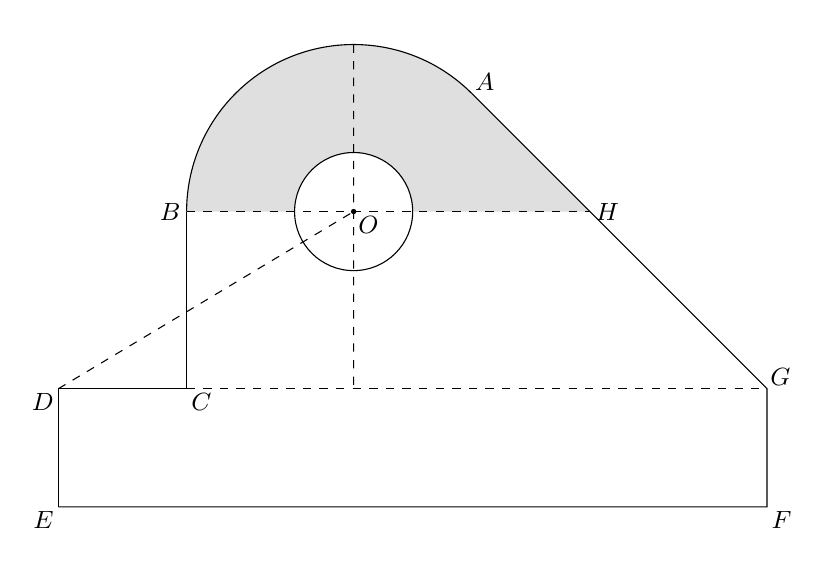
\begin{tikzpicture}[scale=0.75, font=\small]
  \coordinate (D) at (0,2);
  \coordinate (E) at (0,0);
  \coordinate (F) at (12,0);
  \coordinate (G) at (12,2);
  \coordinate (O) at (5,5);
  \coordinate (A) at (7,7);
  \coordinate (B) at (2.1716,5);
  \coordinate (C) at (2.1716,2);
  \coordinate (H) at (9,5);
  \coordinate (T) at (5,7.8284);
  % ---------- 阴影：弧 B→A + AH + HB，随后把圆孔填白 ----------
  \fill[gray!25] (B) arc[start angle=180, end angle=45, radius=2.8284] -- (H) -- cycle;
  \fill[white] (O) circle (1);
  % ---------- 虚线 ----------
  \draw[dashed] (B) -- (H);
  \draw[dashed] (C) -- (G);
  \draw[dashed] (T) -- (5,2);
  \draw[dashed] (D) -- (O);
  % ---------- 实线轮廓与圆孔 ----------
  \draw (E) -- (F) -- (G) -- (A);
  \draw (A) arc[start angle=45, end angle=180, radius=2.8284];
  \draw (B) -- (C);
  \draw (C) -- (D) -- (E);
  \draw (O) circle (1);
  \fill (O) circle (1.3pt);
  % ---------- 标签 ----------
  \node[above right, inner sep=1pt] at (A) {$A$};
  \node[left, inner sep=2pt] at (B) {$B$};
  \node[below right, inner sep=1.5pt] at (C) {$C$};
  \node[below left, inner sep=1.5pt] at (D) {$D$};
  \node[below left, inner sep=1.5pt] at (E) {$E$};
  \node[below right, inner sep=1.5pt] at (F) {$F$};
  \node[above right, inner sep=1pt] at (G) {$G$};
  \node[right, inner sep=2pt] at (H) {$H$};
  \node[below right, inner sep=1.5pt] at (O) {$O$};
\end{tikzpicture}
\end{center}
\nopagebreak[4]
\Needspace{4\baselineskip}
\textbf{解析}

\Needspace{5\baselineskip}
\textbf{第一步，建系。} 以 $E$ 为原点，$EF$ 所在直线为 $x$ 轴、$ED$ 所在直线为 $y$ 轴。由 $EF=12$、$DE=2$ 及 $DEFG$ 为矩形得
\nopagebreak[4]
\[E(0,0),\quad F(12,0),\quad G(12,2),\quad D(0,2).\]

\Needspace{5\baselineskip}
$A$ 到直线 $DE$（即 $y$ 轴）的距离为 $7$，到直线 $EF$（即 $x$ 轴）的距离也为 $7$，故
\nopagebreak[4]
\[A(7,7).\]

\textbf{第二步，定圆心与半径。} 设 $O(x_0,y_0)$。

\begin{itemize}
\item $AG$ 与圆弧相切于 $A$，故 $OA\perp AG$。而 $\overrightarrow{AG}=G-A=(5,-5)\parallel(1,-1)$，于是
\end{itemize}
\nopagebreak[4]
\[(x_0-7)-(y_0-7)=0\ \Longrightarrow\ y_0=x_0 .\]
\begin{itemize}
\item $\angle ODC$ 是 $DO$ 与水平线 $DC$ 的夹角（$C$ 在 $DG$ 上，$DG$ 水平），故
\end{itemize}
\nopagebreak[4]
\[\tan\angle ODC=\frac{y_0-2}{x_0}=\frac35 .\]
把 $y_0=x_0$ 代入：$5x_0-10=3x_0$，得 $x_0=5$。

\Needspace{5\baselineskip}
故
\nopagebreak[4]
\[O(5,5),\qquad R=|OA|=\sqrt{(7-5)^2+(7-5)^2}=2\sqrt2 .\]

\Needspace{5\baselineskip}
\textbf{第三步，定 $B$、$H$。} $BC\perp DG$ 且 $DG$ 水平，故 $BC$ 竖直；$B$ 是切点，故 $OB\perp BC$，即 $OB$ 水平：
\nopagebreak[4]
\[B\left(5-2\sqrt2,\ 5\right),\qquad C\left(5-2\sqrt2,\ 2\right).\]
\Needspace{5\baselineskip}
$BH\parallel DG$ 说明 $H$ 在直线 $y=5$ 上，又 $H$ 在切线 $AG$ 上。切线 $AG$ 上的点可写为 $(7+t,\,7-t)$，令 $7-t=5$ 得 $t=2$：
\nopagebreak[4]
\[H(9,5).\]
于是 $B$、$O$、$H$ 三点共线于 $y=5$，这条线正是阴影区域的下边界。

\textbf{第四步，分割求面积。} 阴影区域由弧 $BA$、线段 $AH$、线段 $HB$ 围成，用 $OA$ 把它分成两块：

\Needspace{5\baselineskip}
① 扇形 $OBA$。$OB$ 指向正西方向（$180^\circ$），$OA$ 方向为 $(2,2)$ 即 $45^\circ$，弧从 $B$ 经最高点到 $A$，圆心角为
\nopagebreak[4]
\[180^\circ-45^\circ=135^\circ=\frac{3\pi}4,\]
\nopagebreak[4]
\[S_1=\frac12R^2\cdot\frac{3\pi}4=\frac12\times8\times\frac{3\pi}4=3\pi .\]

\Needspace{5\baselineskip}
② 直角三角形 $OAH$。因 $OA\perp AH$（切线性质），且
\nopagebreak[4]
\[|OA|=2\sqrt2,\qquad |AH|=\sqrt{(9-7)^2+(5-7)^2}=2\sqrt2,\]
\nopagebreak[4]
\[S_2=\frac12\times2\sqrt2\times2\sqrt2=4 .\]
（核对：$|OH|=9-5=4=\sqrt{8+8}$，与勾股定理一致。）

\Needspace{5\baselineskip}
③ 扣除圆孔。圆孔圆心正是 $O$，而 $O$ 恰落在阴影的下边界 $BH$ 上，故只有\textbf{上半个}圆孔位于阴影区域内：
\nopagebreak[4]
\[S_3=\frac12\pi\times1^2=\frac\pi2 .\]
（半径 $1$ 远小于 $R=2\sqrt2$，且阴影区域恰好覆盖自 $OH$ 经 $OB$、$OA$ 到切线 $AH$ 的整个 $180^\circ$ 扇形范围，故上半圆整个落在阴影内部。）

\Needspace{5\baselineskip}
\textbf{第五步，合成。}
\nopagebreak[4]
\[S=S_1+S_2-S_3=3\pi+4-\frac\pi2=4+\frac{5\pi}2\approx11.854 .\]

填 $4+\dfrac{5\pi}2$。

\gkanswer{答案：$4+\dfrac{5\pi}2$。建系得 $E(0,0)$、$F(12,0)$、$G(12,2)$、$D(0,2)$、$A(7,7)$；由 $OA\perp AG$ 与 $\tan\angle ODC=\dfrac35$ 得 $O(5,5)$、$R=2\sqrt2$、$B\left(5-2\sqrt2,5\right)$、$H(9,5)$，$\angle AOB=135^\circ$；阴影面积 $=\dfrac{135}{360}\pi R^2+\dfrac12\cdot OA\cdot AH-\dfrac12\pi\cdot1^2=3\pi+4-\dfrac\pi2$。}

\end{answer}
\begin{answer}
\gksolhead{16}{}

\textbf{题目}：

已知直四棱柱 $ABCD-A_1B_1C_1D_1$ 的棱长均为 $2$，$\angle BAD=60^\circ$。以 $D_1$ 为球心、$\sqrt5$ 为半径的球面与侧面 $BCC_1B_1$ 的交线长为\gkblank{}。

\Needspace{4\baselineskip}
\textbf{解析}

\Needspace{5\baselineskip}
\textbf{第一步，建系。} 以 $A$ 为原点，$AB$ 为 $x$ 轴，底面内与 $AB$ 垂直的方向为 $y$ 轴，侧棱方向为 $z$ 轴。底面是边长为 $2$、$\angle BAD=60^\circ$ 的菱形，故
\nopagebreak[4]
\[A(0,0,0),\quad B(2,0,0),\quad D(1,\sqrt3,0),\quad C(3,\sqrt3,0),\]
\Needspace{5\baselineskip}
侧棱长为 $2$，
\nopagebreak[4]
\[D_1(1,\sqrt3,2).\]

\Needspace{5\baselineskip}
\textbf{第二步，求 $D_1$ 到侧面 $BCC_1B_1$ 的距离。} 该侧面含 $\overrightarrow{BC}=(1,\sqrt3,0)$ 与竖直方向 $(0,0,1)$，法向量取
\nopagebreak[4]
\[\boldsymbol n=(\sqrt3,-1,0),\]
\Needspace{5\baselineskip}
平面方程为 $\sqrt3x-y-2\sqrt3=0$。于是
\nopagebreak[4]
\[d=\frac{|\sqrt3\times1-\sqrt3-2\sqrt3|}{\sqrt{3+1}}=\frac{2\sqrt3}2=\sqrt3 .\]

\Needspace{5\baselineskip}
\textbf{第三步，定交线圆。} 球半径 $\sqrt5$，故球面与侧面所在平面的交线是圆，其半径
\nopagebreak[4]
\[r=\sqrt{5-3}=\sqrt2,\]
\Needspace{5\baselineskip}
圆心为 $D_1$ 在平面上的射影 $E$。直接验证 $E$ 是 $B_1C_1$ 的中点：$B_1(2,0,2)$、$C_1(3,\sqrt3,2)$ 的中点为 $\left(\dfrac52,\dfrac{\sqrt3}2,2\right)$，而
\nopagebreak[4]
\[\overrightarrow{D_1E}=\left(\frac32,-\frac{\sqrt3}2,0\right),\qquad |\overrightarrow{D_1E}|=\sqrt{\frac94+\frac34}=\sqrt3,\]
且 $\overrightarrow{D_1E}\cdot\overrightarrow{BC}=\dfrac32-\dfrac32=0$，与竖直方向也垂直，故 $D_1E\perp$ 侧面，$E$ 确为圆心。

\Needspace{5\baselineskip}
\textbf{第四步，截取侧面内的弧。} 在侧面内以 $E$ 为原点、沿 $\overrightarrow{BC}$ 方向为 $u$ 轴、沿 $\overrightarrow{B_1B}$ 方向（向下）为 $v$ 轴建立平面直角坐标系，则交线圆为
\nopagebreak[4]
\[u^2+v^2=2,\]
而侧面是矩形 $|u|\leqslant1$（$|BC|=2$，$E$ 为中点）、$0\leqslant v\leqslant2$。圆与两条竖直棱 $u=\pm1$ 交于 $v=\sqrt{2-1}=1$；圆的 $v$ 坐标范围是 $\left[-\sqrt2,\sqrt2\right]$，与 $v=0$ 的交点在 $|u|=\sqrt2>1$（落在矩形外），与 $v=2$ 则根本不相交。

\Needspace{5\baselineskip}
故侧面内的交线是圆上从 $\left(-1,1\right)$ 经 $\left(0,\sqrt2\right)$ 到 $\left(1,1\right)$ 的一段弧，其圆心角为
\nopagebreak[4]
\[2\arctan\frac{1}{1}=90^\circ=\frac\pi2,\]
\Needspace{5\baselineskip}
弧长
\nopagebreak[4]
\[l=r\cdot\frac\pi2=\sqrt2\cdot\frac\pi2=\frac{\sqrt2\pi}2 .\]

填 $\dfrac{\sqrt2\pi}2$。

\gkanswer{答案：$\dfrac{\sqrt2\pi}2$。建系得 $D_1$ 到平面 $BCC_1B_1$ 的距离为 $\sqrt3$，交线圆半径为 $\sqrt{5-3}=\sqrt2$，圆心为 $B_1C_1$ 的中点；该圆被侧面两条竖直棱截得圆心角 $90^\circ$ 的弧，长为 $\sqrt2\cdot\dfrac\pi2=\dfrac{\sqrt2\pi}2$。}

\end{answer}
\begin{answer}
\gksolhead{17}{}

\textbf{题目}：

在 ①$ac=\sqrt3$、②$c\sin A=3$、③$c=\sqrt3b$ 这三个条件中任选一个，补充在下面问题中，若问题中的三角形存在，求 $c$ 的值；若问题中的三角形不存在，说明理由。

问题：是否存在 $\triangle ABC$，它的内角 $A$，$B$，$C$ 的对边分别为 $a$，$b$，$c$，且 $\sin A=\sqrt3\sin B$，$C=\dfrac\pi6$，\gkblank{}？

\Needspace{4\baselineskip}
\textbf{解析}

\Needspace{5\baselineskip}
先处理公共条件。由正弦定理 $\sin A=\sqrt3\sin B$ 得
\nopagebreak[4]
\[a=\sqrt3\,b .\]
\Needspace{5\baselineskip}
再由余弦定理与 $C=\dfrac\pi6$
\nopagebreak[4]
\[\begin{aligned}
c^2&=a^2+b^2-2ab\cos C\\
&=3b^2+b^2-2\cdot\sqrt3b\cdot b\cdot\frac{\sqrt3}2\\
&=4b^2-3b^2=b^2,
\end{aligned}\]
\Needspace{5\baselineskip}
故
\nopagebreak[4]
\[c=b .\]
（顺带可定出三角：由 $A+B=\dfrac{5\pi}6$ 与 $\sin A=\sqrt3\sin B$ 解得 $A=\dfrac{2\pi}3$、$B=\dfrac\pi6$，三内角为 $\dfrac{2\pi}3,\dfrac\pi6,\dfrac\pi6$。）

以下分别补充三个条件。

\gksubpart{条件①：$ac=\sqrt3$}

\Needspace{5\baselineskip}
把 $a=\sqrt3b$、$c=b$ 代入：
\nopagebreak[4]
\[ac=\sqrt3b\cdot b=\sqrt3b^2=\sqrt3\ \Longrightarrow\ b^2=1\ \Longrightarrow\ b=1 .\]
\Needspace{5\baselineskip}
于是
\nopagebreak[4]
\[b=1,\qquad c=1,\qquad a=\sqrt3 .\]
\Needspace{5\baselineskip}
验证：$1+1>\sqrt3$，三边能构成三角形；又
\nopagebreak[4]
\[\cos C=\frac{a^2+b^2-c^2}{2ab}=\frac{3+1-1}{2\sqrt3}=\frac{\sqrt3}2\ \Longrightarrow\ C=\frac\pi6,\]
且 $a=\sqrt3b$ 即正弦定理下的 $\sin A=\sqrt3\sin B$，公共条件全部满足。

故三角形存在，$c=1$。

\gksubpart{条件②：$c\sin A=3$}

\Needspace{5\baselineskip}
由正弦定理 $\dfrac a{\sin A}=\dfrac c{\sin C}$ 得 $\sin A=\dfrac{a\sin C}{c}=\dfrac a{2c}$，于是
\nopagebreak[4]
\[c\sin A=\frac a2=3\ \Longrightarrow\ a=6 .\]
再由 $a=\sqrt3b$ 得 $b=2\sqrt3$，由 $c=b$ 得 $c=2\sqrt3$。

验证：$b+c=4\sqrt3\approx6.93>6=a$，能构成三角形；且 $\sin A=\dfrac a{2c}=\dfrac6{4\sqrt3}=\dfrac{\sqrt3}2$，$c\sin A=2\sqrt3\times\dfrac{\sqrt3}2=3$，与条件相符。

故三角形存在，$c=2\sqrt3$。

\gksubpart{条件③：$c=\sqrt3b$}

\Needspace{5\baselineskip}
公共条件已给出 $c=b$，与 $c=\sqrt3b$ 联立得
\nopagebreak[4]
\[b=\sqrt3b\ \Longrightarrow\ b=0,\]
与 $b>0$ 矛盾；等价地，$c=b$ 与 $c=\sqrt3b$ 要求 $\sqrt3=1$，不可能。

（也可用正弦定理看：$c=\sqrt3b$ 即 $\sin C=\sqrt3\sin B$，而 $\sin C=\dfrac12$，故 $\sin B=\dfrac1{2\sqrt3}=\dfrac{\sqrt3}6\ne\dfrac12=\sin B$，矛盾。）

故这样的三角形不存在。

\textbf{结论}：选① $c=1$；选② $c=2\sqrt3$；选③ 三角形不存在。

\gkanswer{答案：选① $c=1$；选② $c=2\sqrt3$；选③ 三角形不存在。公共条件给出 $a=\sqrt3b$、$c=b$：选①由 $ac=\sqrt3$ 得 $b=1$、$c=1$；选②由 $c\sin A=3$ 得 $a=6$、$b=c=2\sqrt3$；选③要求 $c=\sqrt3b$ 与 $c=b$ 同时成立，只能 $b=0$，矛盾。}

\end{answer}
\begin{answer}
\gksolhead{18}{}

\textbf{题目}：

已知公比大于 $1$ 的等比数列 $\{a_n\}$ 满足 $a_2+a_4=20$，$a_3=8$。

（1） 求 $\{a_n\}$ 的通项公式；

（2） 记 $b_m$ 为 $\{a_n\}$ 在区间 $(0,m]$（$m\in\mathbf N^*$）中的项的个数，求数列 $\{b_m\}$ 的前 $100$ 项和 $S_{100}$。

\Needspace{4\baselineskip}
\textbf{解析}

\gksubpart{（1）}

\Needspace{5\baselineskip}
设首项为 $a_1$、公比为 $q$（$q>1$）。由 $a_3=8$ 得
\nopagebreak[4]
\[a_1q^2=8\ \Longrightarrow\ a_1=\frac8{q^2},\]
\Needspace{5\baselineskip}
代入 $a_2+a_4=20$：
\nopagebreak[4]
\[a_1q+a_1q^3=20\ \Longrightarrow\ \frac8{q^2}\left(q+q^3\right)=20\ \Longrightarrow\ 8\left(\frac1q+q\right)=20 .\]
\Needspace{5\baselineskip}
即
\nopagebreak[4]
\[2q^2-5q+2=0\ \Longrightarrow\ (2q-1)(q-2)=0,\]
故 $q=2$ 或 $q=\dfrac12$。由 $q>1$ 得 $q=2$，于是 $a_1=\dfrac8{4}=2$。

\Needspace{5\baselineskip}
所以
\nopagebreak[4]
\[a_n=2\cdot2^{n-1}=2^n .\]
验算：$a_2+a_4=4+16=20$ ，$a_3=8$ 。

\gksubpart{（2）}

\Needspace{5\baselineskip}
$a_n=2^n$ 关于 $n$ 递增。$b_m$ 是满足 $2^n\leqslant m$ 的正整数 $n$ 的个数，即
\nopagebreak[4]
\[b_m=\left\lfloor\log_2m\right\rfloor .\]
具体地：$m\in\left[2^k,\,2^{k+1}-1\right]$ 时 $b_m=k$（$k=0,1,2,\cdots$）。

$1\leqslant m\leqslant100$ 按 $k$ 分段：

\begin{center}
\begin{tabular}{cccc}
\toprule
$k$ & $m$ 的范围 & 个数 & 贡献 $k\times$个数 \\
\midrule
$0$ & $1$ & $1$ & $0$ \\
$1$ & $2\sim3$ & $2$ & $2$ \\
$2$ & $4\sim7$ & $4$ & $8$ \\
$3$ & $8\sim15$ & $8$ & $24$ \\
$4$ & $16\sim31$ & $16$ & $64$ \\
$5$ & $32\sim63$ & $32$ & $160$ \\
$6$ & $64\sim100$ & $37$ & $222$ \\
\bottomrule
\end{tabular}
\end{center}

\Needspace{5\baselineskip}
故
\nopagebreak[4]
\[S_{100}=0+2+8+24+64+160+222=480 .\]

验算（小规模）：$m=1,\cdots,8$ 时 $b_m=0,1,1,2,2,2,2,3$，前 $8$ 项和为 $13$；按上表 $k\leqslant2$ 部分（$m\leqslant7$）为 $0+2+8=10$，再加 $b_8=3$ 得 $13$ 。

\gkanswer{答案（1）：$a_n=2^n$。由 $a_3=8$ 得 $a_1=\dfrac8{q^2}$，代入 $a_2+a_4=20$ 得 $2q^2-5q+2=0$，$q=2$（舍 $\dfrac12$），$a_1=2$。}

\gkanswer{答案（2）：$480$。$b_m=\left\lfloor\log_2m\right\rfloor$，按 $m$ 所在区间 $[2^k,2^{k+1}-1]$ 分段求和：$0\cdot1+1\cdot2+2\cdot4+3\cdot8+4\cdot16+5\cdot32+6\cdot37=480$。}

\end{answer}
\begin{answer}
\gksolhead{19}{}

\textbf{题目}：

为加强环境保护，治理空气污染，环境监测部门对某市空气质量进行调研，随机抽查了 $100$ 天空气中的 PM2.5 和 $\mathrm{SO_2}$ 浓度（单位：$\mu\mathrm g/\mathrm m^3$），得下表：

\begin{center}
\begin{tabular}{cccc}
\toprule
$\mathrm{SO_2}$ 浓度 & $[0,50]$ & $(50,150]$ & $(150,475]$ \\
\midrule
PM2.5 $[0,35]$ & $32$ & $18$ & $4$ \\
PM2.5 $(35,75]$ & $6$ & $8$ & $12$ \\
PM2.5 $(75,115]$ & $3$ & $7$ & $10$ \\
\bottomrule
\end{tabular}
\end{center}

（1） 估计事件「该市一天空气中 PM2.5 浓度不超过 $75$，且 $\mathrm{SO_2}$ 浓度不超过 $150$」的概率；

（2） 根据所给数据，完成下面的 $2\times2$ 列联表：

\begin{center}
\begin{tabular}{ccc}
\toprule
$\mathrm{SO_2}$ 浓度 & $[0,150]$ & $(150,475]$ \\
\midrule
PM2.5 $[0,75]$ &  &  \\
PM2.5 $(75,115]$ &  &  \\
\bottomrule
\end{tabular}
\end{center}

（3） 根据（2）中的列联表，判断是否有 $99\%$ 的把握认为该市一天空气中 PM2.5 浓度与 $\mathrm{SO_2}$ 浓度有关？

\Needspace{10\baselineskip}
附：$K^2=\dfrac{n(ad-bc)^2}{(a+b)(c+d)(a+c)(b+d)}$，

\begin{center}
\begin{tabular}{cccc}
\toprule
$P(K^2\geqslant k)$ & $0.050$ & $0.010$ & $0.001$ \\
\midrule
$k$ & $3.841$ & $6.635$ & $10.828$ \\
\bottomrule
\end{tabular}
\end{center}

\Needspace{4\baselineskip}
\textbf{解析}

\gksubpart{（1）}

\Needspace{5\baselineskip}
事件「PM2.5 浓度不超过 $75$ 且 $\mathrm{SO_2}$ 浓度不超过 $150$」包含表格左上 $2\times2$ 个格子：
\nopagebreak[4]
\[32+18+6+8=64\ (\text{\text{天}}).\]
\Needspace{5\baselineskip}
用频率估计概率：
\nopagebreak[4]
\[P=\frac{64}{100}=0.64 .\]

\gksubpart{（2）}

按 $75$ 与 $150$ 两个界把原表合并：

\begin{center}
\begin{tabular}{ccc}
\toprule
$\mathrm{SO_2}$ 浓度 & $[0,150]$ & $(150,475]$ \\
\midrule
PM2.5 $[0,75]$ & $32+18+6+8=64$ & $4+12=16$ \\
PM2.5 $(75,115]$ & $3+7=10$ & $10$ \\
\bottomrule
\end{tabular}
\end{center}

即 $a=64$，$b=16$，$c=10$，$d=10$；行合计 $80$、$20$，列合计 $74$、$26$，总计 $100$，与抽查天数一致。

\gksubpart{（3）}

\Needspace{5\baselineskip}
零假设 $H_0$：该市一天空气中 PM2.5 浓度与 $\mathrm{SO_2}$ 浓度无关。由公式
\nopagebreak[4]
\[\begin{aligned}
K^2&=\frac{n(ad-bc)^2}{(a+b)(c+d)(a+c)(b+d)}\\
&=\frac{100\times(64\times10-16\times10)^2}{80\times20\times74\times26}\\
&=\frac{100\times480^2}{3078400}\\
&\approx7.484 .
\end{aligned}\]
\Needspace{5\baselineskip}
查表：$P(K^2\geqslant6.635)=0.010$，$P(K^2\geqslant10.828)=0.001$。因
\nopagebreak[4]
\[6.635<7.484<10.828,\]
故可以在犯错误概率不超过 $0.010$ 的前提下认为二者有关，即有 $99\%$ 的把握认为该市一天空气中 PM2.5 浓度与 $\mathrm{SO_2}$ 浓度有关（但没有 $99.9\%$ 的把握）。

\gkanswer{答案（1）：$0.64$。落在「PM2.5 不超过 $75$ 且 $\mathrm{SO_2}$ 不超过 $150$」的天数为 $32+18+6+8=64$，频率为 $\dfrac{64}{100}=0.64$。}

\gkanswer{答案（2）：$a=64$，$b=16$，$c=10$，$d=10$（列联表见解析正文）。行合计 $80$、$20$，列合计 $74$、$26$。}

\gkanswer{答案（3）：有 $99\%$ 的把握认为二者有关。$K^2=\dfrac{100(64\times10-16\times10)^2}{80\times20\times74\times26}\approx7.484>6.635$，但 $<10.828$。}

\end{answer}
\begin{answer}
\gksolhead{20}{}

\textbf{题目}：

如图，四棱锥 $P-ABCD$ 的底面为正方形，$PD\perp$ 底面 $ABCD$。设平面 $PAD$ 与平面 $PBC$ 的交线为 $l$。
\nopagebreak[4]
\begin{center}% 2020 新高考Ⅰ卷（山东）20：四棱锥 P-ABCD（底面 ABCD 为正方形，PD⊥底面 ABCD）
% 绘制依据：固定源 PDF 原页。底面按斜二测画：A 左前、B 右前、C 右后、D 中后（被遮挡顶点）；
% PD 垂直底面，故 P 画在 D 的正上方（位于版面中偏左）。
% 实线：PA、PB、PC、AB、BC；虚线：PD、AD、DC。只标 P、A、B、C、D 五点。
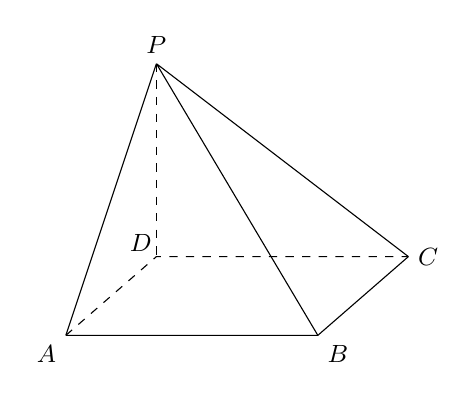
\begin{tikzpicture}[scale=1.0, font=\small]
  \coordinate (A) at (0,0);
  \coordinate (B) at (3.2,0);
  \coordinate (C) at (4.35,1.0);
  \coordinate (D) at (1.15,1.0);
  \coordinate (P) at (1.15,3.45);
  \draw (P) -- (A)  (P) -- (B)  (P) -- (C);
  \draw (A) -- (B) -- (C);
  \draw[dashed] (P) -- (D);
  \draw[dashed] (A) -- (D) -- (C);
  \node[above] at (P) {$P$};
  \node[below left] at (A) {$A$};
  \node[below right] at (B) {$B$};
  \node[right] at (C) {$C$};
  \node[above left, inner sep=1.5pt] at (D) {$D$};
\end{tikzpicture}
\end{center}
\nopagebreak[4]
（1） 证明：$l\perp$ 平面 $PDC$；

（2） 已知 $PD=AD=1$，$Q$ 为 $l$ 上的点，求 $PB$ 与平面 $QCD$ 所成角的正弦值的最大值。

\Needspace{4\baselineskip}
\textbf{解析}

\gksubpart{（1）}

\Needspace{5\baselineskip}
因为 $ABCD$ 是正方形，所以 $BC\parallel AD$。又 $AD\subset$ 平面 $PAD$，$BC\not\subset$ 平面 $PAD$，故
\nopagebreak[4]
\[BC\parallel\text{\text{平面} }PAD .\]
\Needspace{5\baselineskip}
而 $BC\subset$ 平面 $PBC$，且平面 $PAD\cap$ 平面 $PBC=l$，由线面平行的性质定理得
\nopagebreak[4]
\[BC\parallel l .\]

\Needspace{5\baselineskip}
由 $PD\perp$ 底面 $ABCD$，$BC\subset$ 底面，得 $PD\perp BC$；由正方形得 $BC\perp CD$。又 $PD\cap CD=D$，$PD$，$CD\subset$ 平面 $PDC$，故
\nopagebreak[4]
\[BC\perp\text{\text{平面} }PDC .\]
\Needspace{5\baselineskip}
再由 $l\parallel BC$ 得
\nopagebreak[4]
\[l\perp\text{\text{平面} }PDC .\]

\gksubpart{（2）}

\Needspace{5\baselineskip}
以 $D$ 为原点，$\overrightarrow{DA}$，$\overrightarrow{DC}$，$\overrightarrow{DP}$ 分别为 $x$，$y$，$z$ 轴正方向建系。由 $PD=AD=1$、底面为正方形：
\nopagebreak[4]
\[D(0,0,0),\ A(1,0,0),\ C(0,1,0),\ B(1,1,0),\ P(0,0,1).\]

\Needspace{5\baselineskip}
由（1）$l\parallel BC$，而 $\overrightarrow{BC}=(-1,0,0)$，且 $P\in l$，故可设
\nopagebreak[4]
\[Q(t,0,1)\quad(t\in\mathbf R).\]

\Needspace{5\baselineskip}
平面 $QCD$ 由 $\overrightarrow{DC}=(0,1,0)$ 与 $\overrightarrow{DQ}=(t,0,1)$ 张成，法向量
\nopagebreak[4]
\[\boldsymbol n=\overrightarrow{DC}\times\overrightarrow{DQ}=(1\cdot1-0\cdot0,\ 0\cdot t-0\cdot1,\ 0\cdot0-1\cdot t)=(1,0,-t).\]
\Needspace{5\baselineskip}
又
\nopagebreak[4]
\[\overrightarrow{PB}=B-P=(1,1,-1).\]
\Needspace{5\baselineskip}
设 $PB$ 与平面 $QCD$ 所成角为 $\theta$，则
\nopagebreak[4]
\[\sin\theta=\frac{\left|\overrightarrow{PB}\cdot\boldsymbol n\right|}{\left|\overrightarrow{PB}\right|\left|\boldsymbol n\right|}
=\frac{|1+t|}{\sqrt3\sqrt{1+t^2}} .\]

\Needspace{5\baselineskip}
求最大值：对 $t\in\mathbf R$，
\nopagebreak[4]
\[\frac{(1+t)^2}{1+t^2}\leqslant2\iff 1+2t+t^2\leqslant2+2t^2\iff0\leqslant(t-1)^2,\]
\Needspace{5\baselineskip}
恒成立，且 $t=1$ 时取等。故
\nopagebreak[4]
\[\sin\theta\leqslant\frac{\sqrt2}{\sqrt3}=\frac{\sqrt6}3 .\]

即 $PB$ 与平面 $QCD$ 所成角的正弦值的最大值为 $\dfrac{\sqrt6}3$（此时 $Q(1,0,1)$，即 $Q$ 在 $l$ 上使 $DQ=DP$ 的位置）。

\gkanswer{答案（1）：证明。由 $BC\parallel AD$ 得 $BC\parallel$ 平面 $PAD$；又 $BC\subset$ 平面 $PBC$ 且两平面交于 $l$，故 $BC\parallel l$。由 $PD\perp$ 底面得 $PD\perp BC$，正方形给出 $BC\perp CD$，于是 $BC\perp$ 平面 $PDC$，从而 $l\perp$ 平面 $PDC$。}

\gkanswer{答案（2）：$\dfrac{\sqrt6}3$。以 $D$ 为原点建系，$l$ 过 $P(0,0,1)$ 且平行 $BC$，设 $Q(t,0,1)$，平面 $QCD$ 的法向量为 $(1,0,-t)$，$\sin\theta=\dfrac{|1+t|}{\sqrt3\sqrt{1+t^2}}\leqslant\dfrac{\sqrt2}{\sqrt3}=\dfrac{\sqrt6}3$，$t=1$ 时取到。}

\end{answer}
\begin{answer}
\gksolhead{21}{}

\textbf{题目}：

已知函数 $f(x)=a\mathrm e^{x-1}-\ln x+\ln a$。

（1） 当 $a=\mathrm e$ 时，求曲线 $y=f(x)$ 在点 $(1,f(1))$ 处的切线与两坐标轴围成的三角形的面积；

（2） 若 $f(x)\geqslant1$，求 $a$ 的取值范围。

\Needspace{4\baselineskip}
\textbf{解析}

\gksubpart{（1）}

\Needspace{5\baselineskip}
$a=\mathrm e$ 时
\nopagebreak[4]
\[f(x)=\mathrm e\cdot\mathrm e^{x-1}-\ln x+\ln\mathrm e=\mathrm e^x-\ln x+1 .\]
\Needspace{5\baselineskip}
于是
\nopagebreak[4]
\[f(1)=\mathrm e-0+1=\mathrm e+1 .\]
\Needspace{5\baselineskip}
求导：
\nopagebreak[4]
\[f'(x)=\mathrm e^x-\frac1x,\qquad f'(1)=\mathrm e-1 .\]
\Needspace{5\baselineskip}
切线方程为
\nopagebreak[4]
\[y-(\mathrm e+1)=(\mathrm e-1)(x-1)\ \Longrightarrow\ y=(\mathrm e-1)x+2 .\]
\Needspace{5\baselineskip}
它与 $y$ 轴交于 $(0,2)$，与 $x$ 轴交于 $\left(-\dfrac2{\mathrm e-1},0\right)$。故所围三角形面积
\nopagebreak[4]
\[S=\frac12\times2\times\frac2{\mathrm e-1}=\frac2{\mathrm e-1}\approx1.164 .\]

\gksubpart{（2）}

\Needspace{5\baselineskip}
\textbf{必要性。} 取 $x=1$，由 $f(1)=a\cdot\mathrm e^0-\ln1+\ln a=a+\ln a\geqslant1$。函数 $\varphi(a)=a+\ln a$ 在 $(0,+\infty)$ 上严格递增，且 $\varphi(1)=1$，故
\nopagebreak[4]
\[a\geqslant1 .\]

\Needspace{5\baselineskip}
\textbf{充分性。} 设 $a\geqslant1$。则 $\mathrm e^{x-1}>0$ 给出 $a\mathrm e^{x-1}\geqslant\mathrm e^{x-1}$，又 $\ln a\geqslant0$，故
\nopagebreak[4]
\[f(x)=a\mathrm e^{x-1}-\ln x+\ln a\geqslant\mathrm e^{x-1}-\ln x .\]
\Needspace{5\baselineskip}
记 $g(x)=\mathrm e^{x-1}-\ln x$（$x>0$），则
\nopagebreak[4]
\[g'(x)=\mathrm e^{x-1}-\frac1x,\qquad g''(x)=\mathrm e^{x-1}+\frac1{x^2}>0 .\]
\Needspace{5\baselineskip}
故 $g'$ 在 $(0,+\infty)$ 上严格递增；又 $g'(1)=\mathrm e^0-1=0$，所以 $g'<0$ 于 $(0,1)$、$g'>0$ 于 $(1,+\infty)$，$g$ 在 $x=1$ 处取最小值
\nopagebreak[4]
\[g(1)=\mathrm e^0-\ln1=1 .\]
于是 $f(x)\geqslant g(x)\geqslant1$，充分性得证。

综上，$a$ 的取值范围是 $[1,+\infty)$。

（数值复核：$a=1$ 时 $f(1)=1$，且 $x=0.5$ 时 $f=\mathrm e^{-0.5}-\ln0.5\approx0.607+0.693=1.300>1$；$x=3$ 时 $f=\mathrm e^2-\ln3\approx7.389-1.099=6.290>1$，与结论一致。）

\gkanswer{答案（1）：$\dfrac{2}{\mathrm e-1}$。$a=\mathrm e$ 时 $f(x)=\mathrm e^x-\ln x+1$，$f(1)=\mathrm e+1$，$f'(1)=\mathrm e-1$，切线 $y=(\mathrm e-1)x+2$ 的两截距为 $2$ 与 $-\dfrac2{\mathrm e-1}$，面积 $\dfrac12\cdot2\cdot\dfrac2{\mathrm e-1}=\dfrac2{\mathrm e-1}$。}

\gkanswer{答案（2）：$[1,+\infty)$。取 $x=1$ 得必要条件 $a+\ln a\geqslant1$，故 $a\geqslant1$；反之 $a\geqslant1$ 时 $f(x)\geqslant\mathrm e^{x-1}-\ln x\geqslant1$（后者在 $x=1$ 取最小值 $1$）。}

\end{answer}
\begin{answer}
\gksolhead{22}{}

\textbf{题目}：

已知椭圆 $C:\dfrac{x^2}{a^2}+\dfrac{y^2}{b^2}=1$（$a>b>0$）的离心率为 $\dfrac{\sqrt2}2$，且过点 $A(2,1)$。

（1） 求 $C$ 的方程；

（2） 点 $M$，$N$ 在 $C$ 上，且 $AM\perp AN$，$AD\perp MN$，$D$ 为垂足。证明：存在定点 $Q$，使得 $|DQ|$ 为定值。

\Needspace{4\baselineskip}
\textbf{解析}

\gksubpart{（1）}

\Needspace{5\baselineskip}
由离心率
\nopagebreak[4]
\[e=\frac ca=\frac{\sqrt2}2\ \Longrightarrow\ \frac{c^2}{a^2}=\frac12\ \Longrightarrow\ a^2=2c^2 .\]
又 $b^2=a^2-c^2=c^2$，故 $a^2=2b^2$。

\Needspace{5\baselineskip}
代入 $A(2,1)$：
\nopagebreak[4]
\[\frac4{a^2}+\frac1{b^2}=1\ \Longrightarrow\ \frac4{2b^2}+\frac1{b^2}=1\ \Longrightarrow\ \frac3{b^2}=1\ \Longrightarrow\ b^2=3,\ a^2=6 .\]
\Needspace{5\baselineskip}
故
\nopagebreak[4]
\[C:\frac{x^2}6+\frac{y^2}3=1,\qquad\text{\text{即}}\quad x^2+2y^2=6 .\]

\gksubpart{（2）}

设 $M(x_1,y_1)$，$N(x_2,y_2)$。

\Needspace{5\baselineskip}
\textbf{第一步，设直线并联立。} 先设 $MN$ 不垂直于 $x$ 轴，记为 $y=kx+m$。代入 $x^2+2y^2=6$：
\nopagebreak[4]
\[(1+2k^2)x^2+4kmx+2m^2-6=0,\]
\Needspace{5\baselineskip}
故
\nopagebreak[4]
\[x_1+x_2=\frac{-4km}{1+2k^2},\qquad x_1x_2=\frac{2m^2-6}{1+2k^2} .\]

\Needspace{5\baselineskip}
\textbf{第二步，翻译 $AM\perp AN$。} 条件即
\nopagebreak[4]
\[(x_1-2)(x_2-2)+(y_1-1)(y_2-1)=0 .\]
\Needspace{5\baselineskip}
记 $u_i=x_i-2$，$c=m+2k-1$，则 $y_i-1=kx_i+m-1=ku_i+c$，条件化为
\nopagebreak[4]
\[(1+k^2)u_1u_2+kc(u_1+u_2)+c^2=0 .\tag{*}\]
\Needspace{5\baselineskip}
而
\nopagebreak[4]
\[u_1u_2=x_1x_2-2(x_1+x_2)+4=\frac{2\left[(m+2k)^2-1\right]}{1+2k^2},\]
\nopagebreak[4]
\[u_1+u_2=x_1+x_2-4=\frac{-4\left(km+1+2k^2\right)}{1+2k^2} .\]

\Needspace{5\baselineskip}
\textbf{第三步，化简。} 令 $s=m+2k$，则 $c=s-1$，$km+1+2k^2=ks+1$。将 $(*)$ 两边乘 $1+2k^2$：
\nopagebreak[4]
\[2(1+k^2)(s^2-1)-4k(s-1)(ks+1)+(s-1)^2(1+2k^2)=0 .\]
\Needspace{5\baselineskip}
展开合并（$s^2$ 项系数 $2+2k^2-4k^2+1+2k^2=3$，$s$ 项系数 $-4k+4k^2-2-4k^2=-(4k+2)$，常数项 $-2-2k^2+4k+1+2k^2=4k-1$）：
\nopagebreak[4]
\[3s^2-(4k+2)s+(4k-1)=0,\]
\Needspace{5\baselineskip}
即
\nopagebreak[4]
\[(s-1)\left(3s-4k+1\right)=0 .\]

\Needspace{5\baselineskip}
若 $s=1$，则 $m=1-2k$，直线 $y=kx+1-2k$ 过点 $A(2,1)$，此时 $M$ 或 $N$ 与 $A$ 重合，不符合题意，舍去。故
\nopagebreak[4]
\[s=\frac{4k-1}3\ \Longrightarrow\ m=s-2k=-\frac{2k+1}3 .\]
\Needspace{5\baselineskip}
于是
\nopagebreak[4]
\[MN:\ y=kx-\frac{2k+1}3=k\left(x-\frac23\right)-\frac13,\]
\Needspace{5\baselineskip}
它对任意 $k$ 都过定点
\nopagebreak[4]
\[P_0\left(\frac23,-\frac13\right).\]

\Needspace{5\baselineskip}
\textbf{第四步，补上竖直情形。} 若 $MN\perp x$ 轴，设 $MN:x=t$，则 $M$，$N$ 的纵坐标满足 $y_0^2=3-\dfrac{t^2}2$，且
\nopagebreak[4]
\[AM\perp AN\iff(t-2)^2+(y_0-1)(-y_0-1)=0\iff(t-2)^2+1-y_0^2=0 .\]
\Needspace{5\baselineskip}
代入 $y_0^2=3-\dfrac{t^2}2$：
\nopagebreak[4]
\[t^2-4t+4+1-3+\frac{t^2}2=0\ \Longrightarrow\ 3t^2-8t+4=0\ \Longrightarrow\ t=2\ \text{\text{或}}\ t=\frac23 .\]
$t=2$ 时直线过 $A$，舍去；$t=\dfrac23$ 正是过 $P_0$ 的竖直线（$P_0$ 的横坐标为 $\dfrac23$）。故竖直情形同样归结为「$MN$ 过 $P_0$」。

\Needspace{5\baselineskip}
\textbf{第五步，找定点 $Q$。} 由 $AD\perp MN$、$D$ 为垂足、$P_0\in MN$，得
\nopagebreak[4]
\[\angle ADP_0=90^\circ,\]
\Needspace{5\baselineskip}
故 $D$ 在以 $AP_0$ 为直径的圆上。取该圆圆心，即 $AP_0$ 的中点
\nopagebreak[4]
\[Q\left(\frac{2+\frac23}2,\ \frac{1-\frac13}2\right)=\left(\frac43,\ \frac13\right),\]
\Needspace{5\baselineskip}
则该圆半径为
\nopagebreak[4]
\[\frac{|AP_0|}2=\frac12\sqrt{\left(2-\frac23\right)^2+\left(1+\frac13\right)^2}=\frac12\sqrt{\frac{16}9+\frac{16}9}=\frac{2\sqrt2}3 .\]
\Needspace{5\baselineskip}
所以对任意满足条件的 $M$，$N$，都有
\nopagebreak[4]
\[|DQ|=\frac{2\sqrt2}3\quad(\text{\text{定值}}).\]

即存在定点 $Q\left(\dfrac43,\dfrac13\right)$，使得 $|DQ|$ 为定值 $\dfrac{2\sqrt2}3$。

\Needspace{5\baselineskip}
\textbf{数值复核}：取 $k=0$，得 $m=s-2k=-\dfrac13$，即 $MN:y=-\dfrac13$。代入椭圆方程 $x^2+2\cdot\dfrac19=6$ 得 $x=\pm\dfrac{2\sqrt{13}}3$，故
\nopagebreak[4]
\[M\left(\frac{2\sqrt{13}}3,-\frac13\right),\qquad N\left(-\frac{2\sqrt{13}}3,-\frac13\right).\]
\Needspace{5\baselineskip}
于是
\nopagebreak[4]
\[\overrightarrow{AM}\cdot\overrightarrow{AN}=\left(\frac{2\sqrt{13}}3-2\right)\left(-\frac{2\sqrt{13}}3-2\right)+\left(-\frac43\right)\left(-\frac43\right)=\left(4-\frac{52}9\right)+\frac{16}9=0,\]
\Needspace{5\baselineskip}
$AM\perp AN$ 成立。此时 $D$ 为 $A$ 到 $MN$ 的垂足，即 $D\left(2,-\dfrac13\right)$，而
\nopagebreak[4]
\[|DQ|=\sqrt{\left(2-\frac43\right)^2+\left(-\frac13-\frac13\right)^2}=\sqrt{\frac49+\frac49}=\frac{2\sqrt2}3,\]
与所求定值一致。

\Needspace{5\baselineskip}
再取 $k=2$，得 $m=-\dfrac53$，直线 $MN:y=2x-\dfrac53$，先核对它过 $P_0$：$2\times\dfrac23-\dfrac53=-\dfrac13$ 。此时 $A$ 到 $MN$ 的距离为 $\dfrac{|2\times2-1-\frac53|}{\sqrt5}=\dfrac{4}{3\sqrt5}$，垂足
\nopagebreak[4]
\[D=\left(2,1\right)-\frac{4}{3\sqrt5}\cdot\frac{(2,-1)}{\sqrt5}=\left(\frac{22}{15},\frac{19}{15}\right),\]
\nopagebreak[4]
\[|DQ|=\sqrt{\left(\frac{22}{15}-\frac43\right)^2+\left(\frac{19}{15}-\frac13\right)^2}=\sqrt{\frac{4}{225}+\frac{196}{225}}=\sqrt{\frac{200}{225}}=\frac{2\sqrt2}3,\]
再次吻合 。

\gkanswer{答案（1）：$\dfrac{x^2}6+\dfrac{y^2}3=1$。由 $e^2=\dfrac12$ 得 $a^2=2b^2$，代入 $A(2,1)$ 得 $\dfrac4{2b^2}+\dfrac1{b^2}=1$，$b^2=3$。}

\gkanswer{答案（2）：存在定点 $Q\left(\dfrac43,\dfrac13\right)$，使 $|DQ|=\dfrac{2\sqrt2}3$。设 $MN:y=kx+m$，由 $AM\perp AN$ 化简得 $m=-\dfrac{2k+1}3$，即 $MN$ 恒过 $P_0\left(\dfrac23,-\dfrac13\right)$；$AD\perp MN$ 使 $D$ 在以 $AP_0$ 为直径的圆上，取 $Q$ 为 $AP_0$ 中点即得定值 $\dfrac{|AP_0|}2=\dfrac{2\sqrt2}3$。}

\end{answer}